
\documentclass{beamer}
\mode<presentation>
{
  \usetheme{default}      % or try Darmstadt, Madrid, Warsaw, ...
  \usecolortheme{dolphin} % or try albatross, beaver, crane, ...
  \usefonttheme{structurebold}  % or try serif, structurebold, ...
  \setbeamertemplate{navigation symbols}{}
  \setbeamertemplate{caption}[numbered]
} 
\usepackage[english]{babel}  %%%% u¿ywamy przez \selectlanguage
\usepackage[T1]{fontenc}
\usepackage[utf8]{inputenc}
\usepackage{tikz}
\usepackage{pdflscape}
\usepackage{graphicx}
\title[Programowanie Obiektowe]{Gra z gatunku roguelike}

\begin{document}
\begin{frame}
  \titlepage
\end{frame}
\section{Gra}
\begin{frame}{Klasa Game}
Klasa zawiera zmienną stanu gry, ostatni naciśnięty klawisz, oraz zmienną boolowską kontrolującą zegar gry. Moduły:
\begin{itemize}
\item menu - wywoływany na początku, zawiera menu gry
\item game\_loop - główna pętla gry
\item controls - wczytuje klawisze ze standardowego wejścia
\item new\_game - generuje nowy poziom
\item update\_state - przeprowadza odpowiednie akcje w zależności od tego jaki klawisz nacisnął użytkownik
\end{itemize}
\end{frame}
\begin{frame}{Klasa State}
Jest w niej przechowywany gracz, lista potworów oraz aktualna podłoga na której się jest. Moduły:
\begin{itemize}
\item display - wyświetla aktualny stan gry do stdio
\item draw\_ui - rysuje interfejs na wierzchu mapy
\item remove\_dead - usuwa martwe jednostki ze stanu
\item monsters\_to\_tab - zamienia potwory w tablice ich pozycji
\item run\_ai - uruchamia ai wszystkich potworów
\item closest\_monsters - zwraca liste sąsiednich potworów
\item change\_pos - zmienia pozycje gracza
\item attack - atakuje wszystkie potwory naokoło gracza
\end{itemize}
\end{frame}
\begin{frame}{Klasa Player}
Zawiera podstawowe statystyki gracza (życie/mane/poziom/doświadczenie/atak/obronę i inne). Moduły zawarte:
\begin{itemize}
\item generate - generuje nowego gracza
\item set\_pos - ustawia pozycję
\item get\_pos - zwraca pozycję
\item change\_hp - zmienia życie
\item change\_mana - zmienia mane
\item change\_pos - zmienia pozycję o parę
\item add\_exp - dodaje doświadczenie
\item level\_up - zwiększa poziom o 1
\end{itemize}
\end{frame}
\begin{frame}{Klasa Unit}
Zawiera podstawowe statystyki (życie/atak/obronę/pozycję) oraz moduły:
\begin{itemize}
\item pos\_to\_table - zwraca pozycje jednostki relatywnie do gracza
\item get\_pos - zwraca pozycję
\item change\_hp - zmienia życie
\item change\_mana - zmienia mane
\item change\_pos - zmienia pozycję o parę
\item set\_pos - ustawia pozycję
\item run\_ai - uruchamia ai jednostki
\item move\_to - przesuwa jednostke na pole możliwie bliższe graczowi
\end{itemize}
\end{frame}
\begin{frame}{Klasa Floor}
Reprezentuje aktualną mapę na której znajdują się jednostki. Posiada moduły:
\begin{itemize}
\item display - zwraca tablicę podłogi wycentrowaną na graczu
\item change\_tile - zmienia jedno z pól
\item place\_monsters - zwraca listę potworów w wolnych miejscach
\item generate - tworzy nową podłogę
\item carve - wycina korytarze między pokojami
\item generatepoints - generuje punkty na środki pokojów
\end{itemize}
\end{frame}
\begin{frame}{Funkcje globalne}
\begin{itemize}
\item console\_clear - czyści konsole
\item ptos - zamienia parę na stringa z dopełnieniem do prawej
\item ptosr - zamienia parę na stringa z dopełnieniem do lewej
\item addpair - dodaje dwie pary
\item order\_list - sortuje listę wg odległości i zwraca kolejność od najmniejszej do największej
\item neighbours - zwraca listę par sąsiednich do pary wysłanej w argumencie
\item distance - oblicza odległość między dwoma parami
\end{itemize}
\end{frame}
\begin{landscape}
\begin{frame}
\centerline{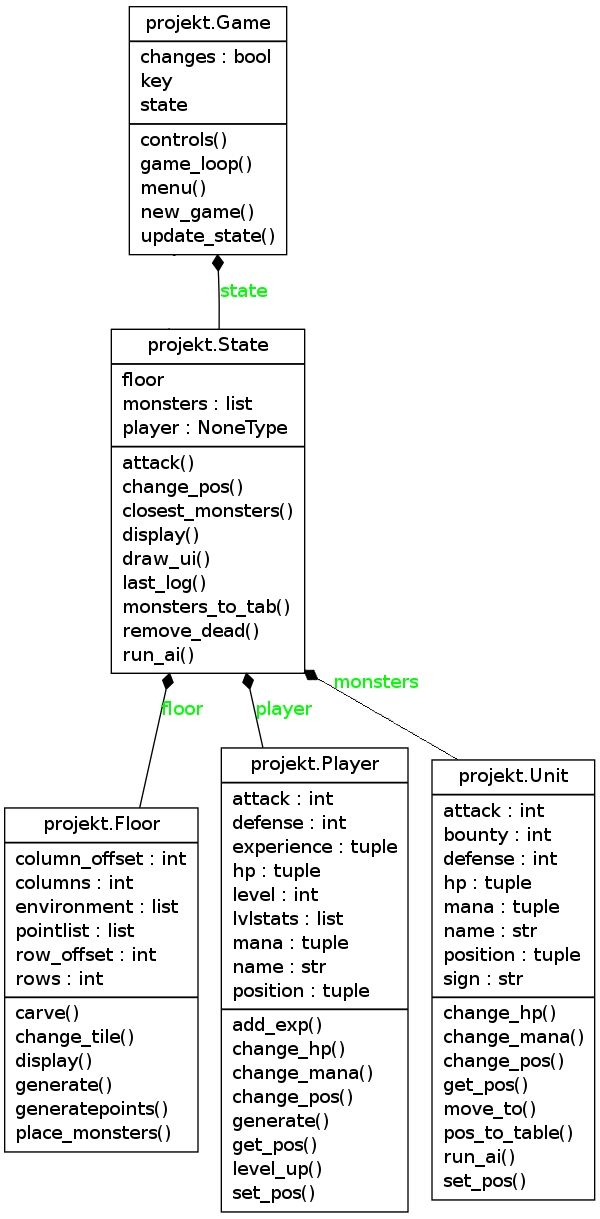
\includegraphics[width=\textwidth,height=\textheight,keepaspectratio]{classes_test.png}}
\end{frame}
\end{landscape}
\begin{frame}
Klasa Unit została zaprogramowana tak że można łatwo dodać dodatkowe rodzaje jednostek, więc łatwo byłoby ją zintegrować w inny, podobny projekt. Gra jako całość mogłaby też zostać włożona do innej, większej gry, jeżeli przechwyciłoby się strumienie wejścia i wyjścia. Klasę Player można użyć ponownie z kosmetycznymi zmianami w innej grze o podobnych właściwościach.
\end{frame}

\end{document}
